\documentclass{standalone}
\usepackage{tikz}

\begin{document}



\tikzset{every picture/.style={line width=0.75pt}} %set default line width to 0.75pt

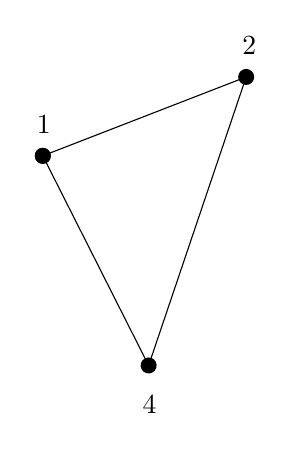
\begin{tikzpicture}[x=0.75pt,y=0.75pt,yscale=-1,xscale=1]
%uncomment if require: \path (0,300); %set diagram left start at 0, and has height of 300

%Straight Lines
\draw    (82.5,88) -- (133.5,189) ;
\draw [shift={(133.5,189)}, rotate = 63.21] [color={rgb, 255:red, 0; green, 0; blue, 0 }  ][fill={rgb, 255:red, 0; green, 0; blue, 0 }  ][line width=0.75]      (0, 0) circle [x radius= 3.35, y radius= 3.35]   ;
\draw [shift={(82.5,88)}, rotate = 63.21] [color={rgb, 255:red, 0; green, 0; blue, 0 }  ][fill={rgb, 255:red, 0; green, 0; blue, 0 }  ][line width=0.75]      (0, 0) circle [x radius= 3.35, y radius= 3.35]   ;
%Straight Lines
\draw    (82.5,88) -- (180.5,50) ;
\draw [shift={(180.5,50)}, rotate = 338.81] [color={rgb, 255:red, 0; green, 0; blue, 0 }  ][fill={rgb, 255:red, 0; green, 0; blue, 0 }  ][line width=0.75]      (0, 0) circle [x radius= 3.35, y radius= 3.35]   ;
\draw [shift={(82.5,88)}, rotate = 338.81] [color={rgb, 255:red, 0; green, 0; blue, 0 }  ][fill={rgb, 255:red, 0; green, 0; blue, 0 }  ][line width=0.75]      (0, 0) circle [x radius= 3.35, y radius= 3.35]   ;
%Straight Lines
\draw    (133.5,189) -- (180.5,50) ;



% Text Node
\draw (83,73) node   {$1$};
% Text Node
\draw (134,208) node   {$4$};
% Text Node
\draw (182,35) node   {$2$};


\end{tikzpicture}

\end{document}
